%% !TEX root = ../Thesis.tex
%% !TEX output_directory
\documentclass[11pt,a4paper,english,greek,twoside]{../Thesis}
\usepackage{mathtools}  
\mathtoolsset{showonlyrefs}  
\begin{document}
%\everymath{\displaystyle}
\chapter{Θεωρητικό υπόβαθρο}\label{chap:Background}
\par Σε αυτό το κεφάλαιο θα παρουσιαστούν όλες οι υπολογιστικές μέθοδοι που χρησιμοποιήθηκαν σε αυτήν την διπλωματική εργασία, και που αφορούν την προ-επεξεργασία των εγκεφαλικών σημάτων, την εξαγωγή κατάλληλων-αντιπροσωπευτικών χαρακτηριστικών από τα σήματα, τα οποία θα χρησιμοποιηθούν ως είσοδος στους αλγορίθμους απόφασης και μηχανικής μάθησης. Σε αυτό το επίπεδο θα γίνει μόνο μια αναφορά στα γενικά χαρακτηριστικά της κάθε μεθόδου, οπότε είναι πιθανό να μην γίνει άμεσα αντιληπτός ο συγκεκριμένος τρόπος με τον οποίον θα εφαρμοστεί η κάθε μέθοδος στο παρών πρόβλημα. Αυτού του είδους η ανάλυση θα γίνει στις υποενότητες \ref{subsec:preprocessing} και \ref{subsec:featureExtract}
\section{Αποθορυβοποίηση - Φιλτράρισμα}
\subsection{Είδη Φίλτρων}
Γενικά η λειτουργία ενός φίλτρου μπορεί να χαρακτηριστεί από τη χαρακτηριστική του απόκριση στο πεδίο του χρόνου. Πιο συγκεκριμένα, οι πιο συχνά χρησιμοποιούμενες κατηγορίες αφορούν φίλτρα τα οποία επιτρέπουν την διέλευση συχνοτήτων από ένα κατώφλι και άνω, όπου ονομάζονται υψιπερατά, ενώ από ένα κατώφλι και κάτω, βαθυπερατά. Τέλος υπάρχουν και αυτά που είτε επιτρέπουν την διέλευση μεταξύ δύο προκαθορισμένων συχνοτήτων (ζωνοπερατά), είτε την εμποδίζουν (φραγμού-ζώνης).
\begin{figure}[H]
    \centering     %%% not \center
    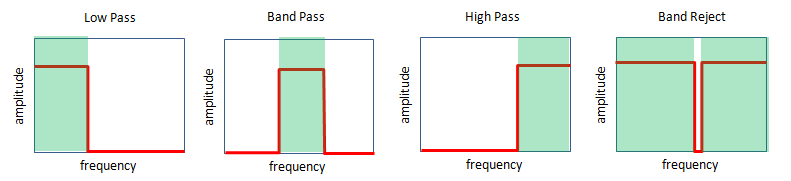
\includegraphics[scale=0.7]{{ImagesSSVEP/filter_types}.png}
    \caption{Τα τέσσερα βασικά είδη φίλτρων με βάση τις ζώνες συχνοτήτων που επιτρέπουν-απορρίπτουν. Αξίζει να σημειωθεί πως οι υποφαινόμενες αποκρίσεις στο πεδίο της συχνότητας, αναφέρονται σε ιδανικά φίλτρα (brick-wall filters), και πως στα πραγματικά, οι ζώνες αποκοπής δεν ορίζονται ποτέ από κάθετες γραμμές.}
    \label{fig:filter_types}
\end{figure}
\par Ένα άλλο κριτήριο με βάση το οποίο διαχωρίζονται τα φίλτρα είναι ο τρόπος με τον οποίο κάθε στιγμή χειρίζονται τις προηγούμενες εισόδους και εξόδους του συστήματος. Τα φίλτρα των οποίων η έξοδος εξαρτάται μόνο από τις προηγούμενες εισόδους ονομάζονται Φίλτρα Πεπερασμένης Κρουστικής Απόκρισης (Finite Impulse Response - FIR), ενώ αυτά που λαμβάνουν υπόψιν τους τόσο τις προηγούμενες εισόδους, αλλά και τις προηγούμενες εξόδους ονομάζονται Φίλτρα Άπειρης Κρουστικής Απόκρισης (Infinite Impulse Response - IIR). Το γεγονός πως τα IIR χρησιμοποιούν ένα είδος ανάδρασης (εξάρτηση από προηγούμενες εισόδους) είναι δυνατόν να τα καταστήσει ασταθή, πράγμα το οποίο δεν συμβαίνει με τα FIR, αν όμως χρησιμοποιηθεί με σωστό τρόπο, τότε, δεδομένων κάποιων συγκεκριμένων προδιαγραφών για ένα φίλτρο, μια IIR υλοποίηση θα ικανοποιήσει τις προδιαγραφές κάνοντας χρήση φίλτρου τάξης πολύ χαμηλότερης από το αντίστοιχο FIR, το οποίο μεταφράζεται σε λιγότερες πράξεις, άρα και σε λιγότερο υπολογιστικό χρόνο. 

\par Ένα από τα πιο κλασσικά IIR φίλτρα σχεδιάστηκε το 1930 απο το βρετανό μηχανικό και φυσικό Stephen Butterworth \cite{}. Βασικός στόχος του φίλτρου αυτού ήταν η επίτευξη σταθερής απόκρισης στη περιοχή διέλευσης συχνοτήτων, σε αντίθεση με τα μέχρι τότε φίλτρα τα οποία εμφάνιζαν διακυμάνσεις στην απόκρισή τους (ripple). Το τίμημα όμως για αυτήν την συμπεριφορά, είναι πως υπάρχει σχετικά μεγάλη απόκλιση στην περιοχή της συχνότητας αποκοπής, συγκριτικά με την απόκριση του αντίστοιχου ιδανικού φίλτρου.
\begin{figure}[H]
    \centering     %%% not \center
    \noindent\makebox[\textwidth]{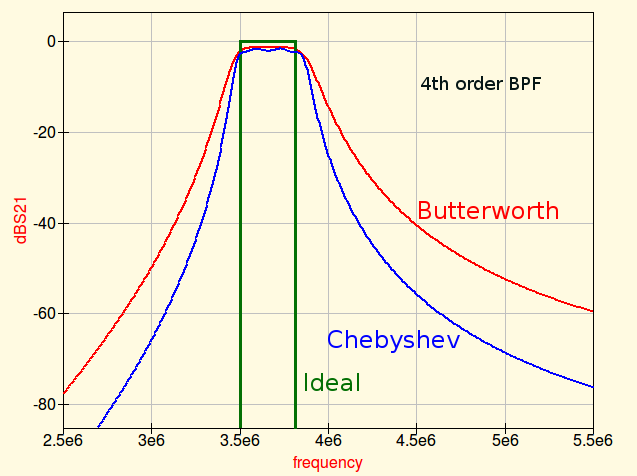
\includegraphics[scale=0.6]{{ImagesSSVEP/butter_cheby}.png}}
    \caption{Οι τρείς διαφορετικές αποκρίσεις για δύο διαφορετικά φίλτρα 3ης τάξης και του αντίστοιχου ιδανικού. Φαίνεται ξεκάθαρα η διακύμανση (ripple) στην ζώνη διέλευσης για ένα φίλτρο τύπου Chebyshev, η οποία δεν υπάρχει στο Butterwoth, καθώς και η μεγάλη απόκλιση του Butterworth σε σχέση με το ιδανικό, όσον αφορά τις δύο ζώνες αποκοπής. }
    \label{fig:butter_cheby}
\end{figure}
% add butte2
\section{Εξαγωγή χαρακτηριστικών}
\subsection{Canonical Correlation Analysis - CCA}

\par Η CCA είναι μια στατιστική μέθοδος που χρησιμοποιείται για την ανάλυση δομών δεδομένων, και συγκεκριμένα για την ανίχνευση της ομοιότητας μεταξύ δύο συνόλων μεταβλητών. Αυτό επιτυγχάνεται μέσω της εύρεσης δύο νέων συνόλων μεταβλητών, όπου το καθένα είναι γραμμικός συνδυασμός ενός από τα αρχικά σύνολα, έτσι ώστε να μεγιστοποιείται ο συντελεστής συσχέτισης τους. Κάνοντας χρήση μαθηματικού φορμαλισμού, έστω  
\section{Μηχανική Μάθηση}

\subsection{Principal Component Analysis - PCA}
\par Η Ανάλυση Κυρίων Συνιστωσών είναι μια στατιστική μέθοδος, που στο τομέα της μηχανικής μάθησης χρησιμοποιείται πολύ συχνά για την ελάττωση των χαρακτηριστικών (features) των δειγμάτων ενός συνόλου, επιλέγοντας μόνο εκείνα τα χαρακτηριστικά τα οποία συνεισφέρουν στην διατήρηση του μεγαλύτερου ποσοστού της μεταβλητότητας (variance) του συνόλου. Μια γεωμετρική ερμηνεία της παραπάνω διαδικασίας, είναι η προσπάθεια εύρεσης των κατευθύνσεων - αξόνων μέγιστης μεταβλητότητας των δεδομένων, και η προβολή τους σε κάποιους από αυτούς τους άξονες.
%ΕΙΚΟΝΑ 4 sub figures

\par Η χρησιμότητα της μεθόδου αυτής είναι εμφανής όταν έχουμε πολυδιάστατα δείγματα, όπως για παράδειγμα εικόνες  μεγέθους 16x16, δηλαδή δυανύσματα χαρακτηριστικών που ανήκουν στο $R^{256}$. Η χρήση όλων αυτών των χαρακτηριστικών σε έναν ακριβά υπολογιστικό αλγόριθμο μηχανικής μάθησης, όπως ο k-NN, θα επιβάρυνε σημαντικά την διαδικασία απόφασης, τόσο υπολογιστικά όσο και χρονικά. Με την χρήση της PCA όμως, είναι δυνατό να επιλεχθεί ένας αριθμός χαρακτηριστικών (π.χ 50-60), τα οποία να διατηρούν την πιο σημαντική στατιστική πληροφορία του συνόλου των εικόνων, με αποτέλεσμα να ελαττώνονται σημαντικά οι πόροι που χρείαζονται για την ταξινόμηση τους, χωρίς την εισαγωγή σημαντικού σφάλματος ταξινόμησης. Τέλος, ένα επιπλέον πλεονέκτημα, είναι πως σε πολλές περιπτώσεις, η PCA, βοηθάει στην αποφυγή του overfitting.

\par Όσον αφορά τον τρόπο υπολογισμού των κύριων συνιστωσών, θα δώσουμε ένα παράδειγμα, για ένα σύνολο δειγμάτων $X$ όπου το καθένα έχει δύο χαρακτηριστικά, δηλαδή $X_i \epsilon R^2$, όπου ο σκοπός μας είναι να του ελαττώσουμε την διάσταση κατά ένα. Αρχικά υπολογίζουμε τον πίνακα 
\begin{align}
\Sigma = \frac{1}{m}\sum_{i=1}^{i=m} X_i(X_i)^T \label{eq1}
\end{align}

\par Υποθέτοντας πως τα δεδομένα μας είναι κανονικοποιημένα έτσι ώστε $E[X_i]=0$ τότε η \eqref{eq1} ορίζει τον πίνακα συνδιασποράς του συνόλου $X$. Αποδεικνύεται πως η κατεύθυνση μέγιστης μεταβλητότητας $u_1$ (βλεπε εικόνα) αντιστοιχεί στο ιδιοδιάνυσμα που προκύπτει από την μεγαλύτερη ιδιοτιμή του πίνακα $\Sigma$. Αντίστοιχα η αμέσως επόμενη κατεύθυνση μέγιστης μεταβλητότητας $u_2$, αντιστοιχεί στο ιδιοδιάνυσμα που προκύπτει από την αμέσως μικρότερη ιδιοτιμή. Γενικεύοντας τώρα την παραπάνω πρόταση, αν τα δεδομένα μας $X_i \epsilon R^n$, και θέλουμε να τα προβάλουμε σε έναν υποχώρο διάστασης $R^k$, $k<n$, τότε πρέπει να διαλέξουμε τα $u_1,...,u_k$ να είναι τα ιδιοδιανύσματα που προκύπτουν από τις $k$ μεγαλύτερες ιδιοτιμές του πίνακα $\Sigma$, ο οποίος επειδή είναι συμμετρικός, τότε τα $u_i$, μπορούν πάντα να επιλέγονται έτσι ώστε να σχηματίζουν μια νέα ορθογώνια βάση για τα δεδομένα.

\par Στην συνέχεια του παραδείγματος μας τώρα, αφού υπολογίσουμε τα δύο ιδιοδιανύσματα $u_1$ και $u_2$ τότε μπορούμε να αναπαραστήσουμε τον πίνακα δεδομένων $X$, ως προς την ορθογώνια βάση $(u_1,u_2)$
\begin{align}
X_{rot} = U^TX =\begin{bmatrix}u_1^T\\u_2^T\end{bmatrix}X= \begin{bmatrix}u_1^TX\\u_2^TX\end{bmatrix}
\label{eq2}
\end{align}
\end{document}
